\documentclass[a4paper,10pt]{article}
\usepackage[utf8]{inputenc}
\usepackage[spanish]{babel}
\usepackage[hmargin=2.5cm, vmargin=2.5cm]{geometry}
\usepackage{amsmath}
\usepackage{graphicx}
\usepackage{subcaption} % enables subfigure
\usepackage{multicol}
\usepackage{natbib}
\setlength{\bibsep}{0.0pt}      % shrink spaces in references
\usepackage{url}
\usepackage[pdftex,colorlinks=true]{hyperref}
\hypersetup{
    allcolors=black,
}
\usepackage{mathptmx} %Times font


\title{
    \textbf{
    TESSEROIDES CON DENSIDADES VARIABLES:
    CÁLCULO DE CAMPOS GRAVITATORIOS EN COORDENADAS ESFÉRICAS CON
    DENSIDADES VARIABLES EN PROFUNDIDAD
    }
}
\author{
    Santiago R. Soler$^{1,2}$ \vspace{0.5em} \\ 
    \normalsize{\textit{$^1$ Instituto Geofísico Sismológico Volponi, Universidad Nacional de San Juan}} \\
    \normalsize{\textit{$^2$ Consejo Nacional de Investigaciones Científicas y Técnicas (CONICET)}} \vspace{0.4em} \\
    \normalsize{email: santiago.r.soler@gmail.com}
}
\date{}


\begin{document}

\renewcommand{\tablename}{Tabla}

\maketitle

\vspace{-2.5em}
\begin{center}
\textbf{Palabras Clave:} gravimetría, tesseroid, densidad variable
\end{center}
\vspace{0.5em}

\begin{abstract}
El cálculo directo de campos gravitatorios para grandes extensiones requiere tomar en cuenta la curvatura de la Tierra, lo cual suele resolverse a través del uso de prismas esféricos llamados Tesseroides.
Además, muchas estructuras geológicas presentan variaciones de la densidad con la profundidad.
En este trabajo hemos sido capaces de implementar un modelo directo que reproduce los campos gravitatorios generados por Tesseroides con densidad variable en profundidad, para lo cual hemos utilizado como aproximación la Cuadratura de Gauss-Legendre y un algoritmo de discretización adaptativa con el objetivo de garantizar la precisión de la misma.
El código fue escrito en Python y Cython y será liberado como Software Libre.

\end{abstract}


\section{Introducción}

Las variaciones de la densidad en la corteza con la profundidad han sido estudiadas por casi un siglo: se propusieron diferentes tipos de variaciones con la profundidad \citep{Athy1930, Maxant1980, Rao1986, Rao1993, Rao1994} e incluso se han tenido en cuenta en modelos directos y de inversión gravimétrica, principalmente aplicados en cuencas y fosas \citep{Cordell1973, Rao1986, Cowie1990, Rao1993, Rao1994, Zhang2001, Welford2010}.

Estos modelos directos fueron desarrollados para cuerpos bidimensionales o tridimensionales en coordenadas cartesianas, los cuales se ajustan adecuadamente para aplicaciones de escalas locales.
Sin embargo, la disponibilidad de datos gravimétricos satelitales permite llevar a cabo estudios e interpretaciones a escalas regionales, en las cuales es necesario tomar en cuenta la curvatura de la Tierra a la hora de realizar modelados directos. 


\begin{figure}
    \begin{subfigure}[t]{0.5\textwidth}
    \centering
    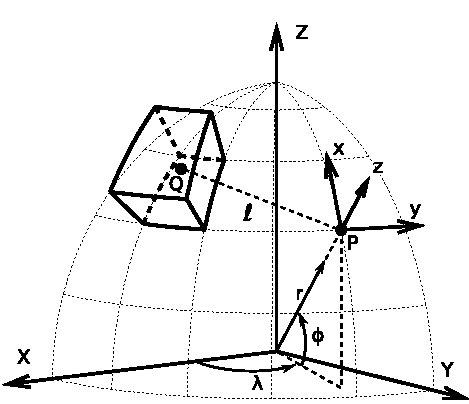
\includegraphics[height=18em]{../manuscript/figures/tesseroid-uieda.pdf}
    \caption{
        Prisma esférico, también conocido como Tesseroide, en un sistema geocéntrico de coordenadas esféricas, junto a un punto de cómputo $P$ y su respectivo sistema de coordenadas Cartesiano local orientado hacia el Norte. Imágen producida por \citet{Uieda2015}.
    }
    \label{fig:tesseroid-uieda}
    \end{subfigure}
    \quad
    \begin{subfigure}[t]{0.5\textwidth}
    \centering
    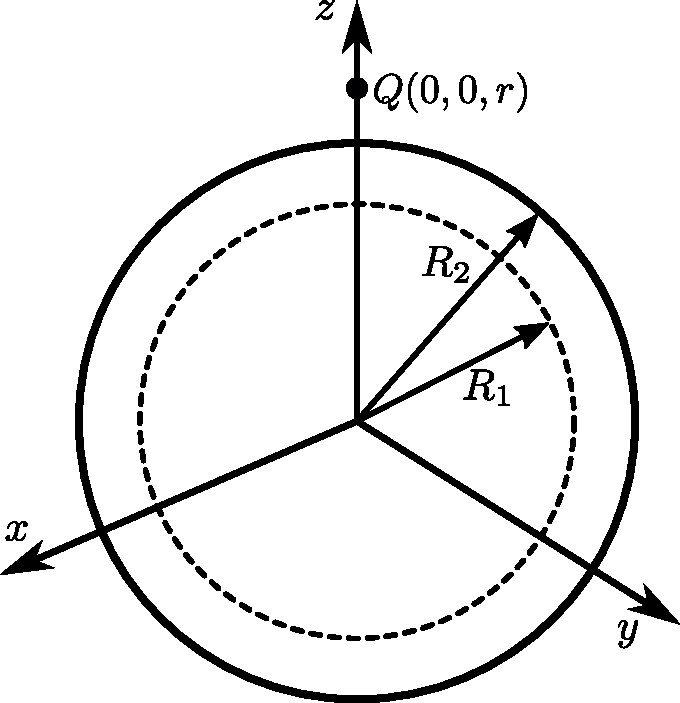
\includegraphics[height=18em]{../manuscript/figures/spherical-shell.pdf}
    \caption{
        Cascarón esférico con radios interior y exteior $R_1$ y $R_2$, respectivamente. El punto de cómputo $Q$ está localizado en el eje $z$ a una distancia $r$ al centro del cascarón. Vamos a suponer que $Q$ se encuentra por fuera del radio exterior $R_2$, es decir $r > R_2$.
    }
    \label{fig:spherical-shell}
    \end{subfigure}
    \caption{}
\end{figure}

Un método muy común para hacerlo es discretizar la Tierra en prismas esféricos conocidos como Tesseroides (ver Figura \ref{fig:tesseroid-uieda}).
El cómputo de campos gravitatorios generados por un tesseroide arbitrario en un punto externo al mismo involucra la resolución de integrales volumétricas.
En caso de que el tesseroide posea una densidad variable, las ecuaciones obtenidas por \citet{Grombein2013} \citep[ver también][]{Uieda2016} para el cómputo de los campos gravitatorios se ven ligeramente modificadas. Por ejemplo, el potencial generado por un tesseroide arbitrario con densidad $\rho(r')$ sobre un punto de cómputo $P(r, \phi, \lambda)$ se puede obtener como:

\begin{equation}
    V(r,\phi,\lambda) = G 
    \int\limits_{\lambda_1}^{\lambda_2}
    \int\limits_{\phi_1}^{\phi_2}
    \int\limits_{r_1}^{r_2}
    \frac{\rho(r')}{\sqrt{{r'}^2 + r^2 - 2 r' r \cos \psi}} \, 
    r'^2 \cos \phi  dr' d\phi' d\lambda',
\label{eq:tesseroid-pot}
\end{equation}
\noindent donde
\begin{equation}
    \cos\psi = \sin\phi\sin\phi' + \cos\phi\cos\phi'
                 \cos(\lambda' - \lambda).
\label{eq:cospsi}
\end{equation}

Este tipos de integrales son generalmente aproximadas por cálculos numéricos.
Para el caso de densidades variables hemos concluido que uno de los métodos que mejor se adecúa para hacerlo es el que involucra la utilización de la Cuadratura de Gauss Legendre (GLQ) \citep{Asgharzadeh2007, Uieda2016, Uieda2017}.
El mismo consiste en aproximar las integrales por una suma ponderada de los efectos de masas puntuales localizadas en los ceros (previamente rescaldados) de los polinomios de Legendre:

\begin{equation}
    \iiint\limits_\Omega \rho(r') g(r', \phi', \lambda') d\Omega \approx
    A 
    \sum\limits_{i=1}^{N^r}
    \sum\limits_{j=1}^{N^\phi}
    \sum\limits_{k=1}^{N^\lambda}
    W_i^r W_j^\phi W_k^\lambda \rho(r_i) g(r_i, \phi_j, \lambda_k),
\label{eq:glq-var-dens}
\end{equation}
\noindent donde
\begin{equation}
    g(r', \phi', \lambda') =
    \frac{r'^2 \cos \phi}{\sqrt{{r'}^2 + r^2 - 2 r' r \cos \psi}},
    \quad
    W_i = \frac{2}{(1-x_i^2)[P_N^\prime(x_i)]^2},
    \quad
    A = \frac{(\lambda_2 - \lambda_1)(\phi_2 - \phi_1)(r_2 - r_1)}{8},
\end{equation}

\noindent $P_N$ es el polinomio de Legendre de orden $N$, $x_i$ sus ceros y $N^i$ con $i \in \{ r, \phi, \lambda\}$ los órdenes de las aproximaciones GLQ.

\citet{Uieda2016} desarrollaron un modelo directo que permite calcular los campos gravitatorios generados por tesseroides con densidad homogenea utilzando las GLQ, implementado en Python e incluido en la librería de código abierto Fatiando a Terra \citep{Uieda2013} para el modelado e inversión geofísica.

\citet{Ku1977} advirtió que la aproximación GLQ se vuelve menos precisa a medida que el punto de cómputo se acerca al tesseroide o bien para órdenes menores de GLQ.
En vez de aumentar los órdenes de la aproximación, \citet{Uieda2016} lo fijan a segundo orden y aumentan la precisión a través de una versión modificada del algoritmo de discretización adaptativa de \citet{Li2011}.
Este consiste en dividir al tesseroide en otros más pequeños en caso de que el cociente entre $d$ y $L_i$ es menor a un valor predefinido $D$ llamado relación distancia-tamaño, donde $d$ es la distancia entre el punto de cómputo y el centro del tesseroide, mientras $L_i$ son las dimensiones del mismo ($i \in \{ r, \phi, \lambda\}$).

De esta manera, el valor asignado a $D$ controla la precisión de la aproximación: para mayores valores de $D$, el error de la aproximación se reduce.
Sin embargo, no existe una relación directa entre $D$ y dicho error.
Es por ello que \citet{Uieda2016} obtuvieron valores estándar de $D$ comparando los campos gravitatorios generados por un cascarón esférico con densidad constante, un caso especial de las integrales volumétricas que posee solución analítica \citep{LaFehr1991, Mikuska2006, Grombein2013}.

En este trabajo hemos implementado un modelo directo como el de \citet{Uieda2016} que además permite calcular los campos gravitatorios generados por tesseroides con densidades variables arbitrarias en profundidad.
Al igual que el anterior, hace uso de la aproximación GLQ, de la versión modificada del algoritmo de discretización adaptativa y su implementación está escrita en lenguajes Python y Cython.

Para garantizar la precisión de la aproximación numérica, hemos llevado a cabo pruebas similares a las que realizaron \citet{Uieda2016} comparando los resultados del modelo numérico con las soluciones analíticas de un cascarón esférico, en nuestro caso con densidades lineales y exponenciales.
Para lo cual fue necesario obtener las soluciones analíticas correspondientes a cada función de densidad.


\section{Determinación de Relación Distancia-Tamaño}

Con el objetivo de evaluar el nuevo modelo directo con tesseroides de densidad variable y estimar el error de la aproximación hemos comparado el modelo numérico con las soluciones analíticas de un cascarón esférico para dos casos especiales: una densidad linear y una exponencial

La estimación del error nos es útil para la determinación del mínimo valor de relación distancia-tamaño $D$ de manera tal que la diferencia entre el modelo numérico y las soluciones analíticas estén debajo de un umbral aceptable.

Hemos aproximado el cascarón esférico a través de una malla de tesseroides de $30^\circ \times 30^\circ$ para luego calcular el potencial gravitatorio, la componente vertical del gradiente $g_z$ y la componente diagonal del tensor de Marussi $g_{zz}$ que la malla genera sobre cuatro grillas: (1) una localizada en el polo, (2) otra en el Ecuador, (3) una localizada a altura satelital y (4) una gran grilla de $30^\circ \times 30^\circ$.
En la Tabla \ref{tab:grids} podemos obtener más información acerca de estas grillas.

Además, el cómputo de estos campos gravitatorios en cada punto de estas grillas fue realizado para diferentes valores de $D$: desde 0.5 a 10 con un paso de 0.5, para luego calcular la máxima diferencia entre estos resultados y el valor de la solución analítica a la misma altura.
Finalmente obtenemos como valor aceptable de $D$ el que presente un error de la correspondiente aproximación numérica menor a 0.1\%.

\begin{figure}[b!]
    \begin{subfigure}[t]{0.5\textwidth}
    \centering
    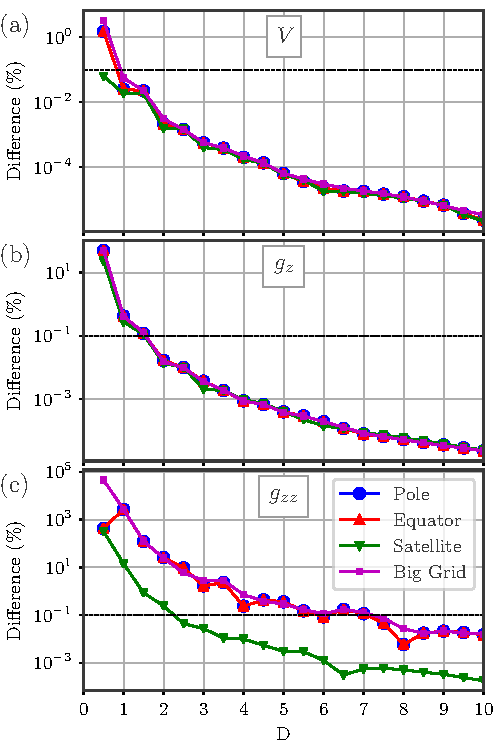
\includegraphics[height=30em]{../manuscript/figures/Dlinear-thin-differences.pdf}
    \caption{}
    \label{fig:D-linear-thin}
    \end{subfigure}
    \quad
    \begin{subfigure}[t]{0.5\textwidth}
    \centering
    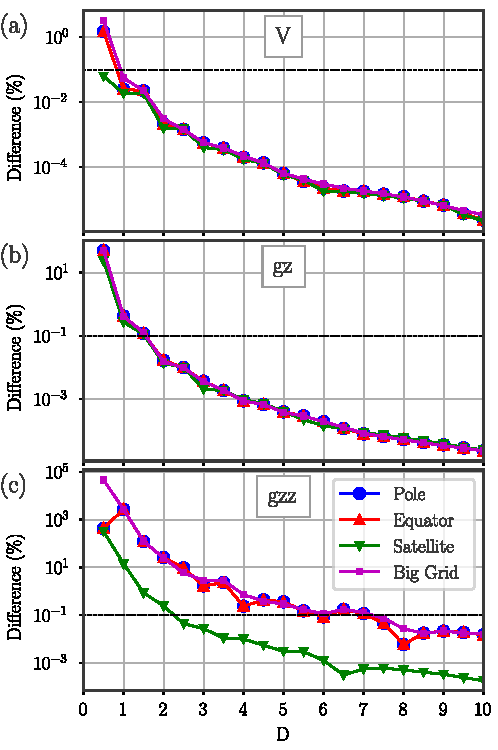
\includegraphics[height=30em]{../manuscript/figures/Dexp-shifted-thin-differences.pdf}
    \caption{}
    \label{fig:D-exp-thin}
    \end{subfigure}
    \caption{
        Diferencias entre los campos gravitatorios generados por el modelo numérico y la solución analítica para un cascarón esférico de 1km de grosor con (a) densidad lineal definida en la ecuación \ref{eq:density-linear} y (b) densidad exponencial definida en la ecuación \ref{eq:density-exp}. Los computos fueron realizados en las cuatro grillas descriptas en la Tabla \ref{tab:grids} y para diferentes valores de la relación distancia-tamaño $D$. Si la diferencia es menor a 0.1\% consideraremos que el modelo ha alcanzado una precisión aceptable para el valor correspondiente de $D$.
    }
\end{figure}


\begin{table}
\centering
\caption{
    Descripciones de las grillas sintéticas en las cuales la comparación entre el modelo numérico y las soluciones analíticas se lleva a cabo. Esta colección de grilla intenta incluir todo posible escenario en el cual el modelo numérico pueda presentar diferentes comportamientos, dependiendo del tamaño de la grilla, su ubicación o su altura sobre la superficie de la Tierra. Cada grilla consiste en un conjunto de 10$\times$10 puntos.
}
\label{tab:grids}
\begin{tabular}{lcccc}
    Grilla & Tamaño & Extensión Lat. & Extensión Lon. & Altura \\ \hline
    Pole & $1^\circ \times 1^\circ$ & $89^\circ - 90^\circ$ & $0^\circ - 1^\circ$ & 2km \\
    Equator & $1^\circ \times 1^\circ$ & $0^\circ - 1^\circ$ & $0^\circ - 1^\circ$ & 2km \\
    Satellite & $1^\circ \times 1^\circ$ & $89^\circ - 90^\circ$ & $0^\circ - 1^\circ$ & 260km \\
    Big Grid & $30^\circ \times 30^\circ$ & $60^\circ - 90^\circ$ & $0^\circ - 30^\circ$ & 2km \\
\end{tabular}
\end{table}

Este proceso de determinación de $D$ fue realizado para una función lineal (ecuación \ref{eq:density-linear}) y una exponencial (ecuación \ref{eq:density-exp}), cuyos resultados pueden observarse en las Figuras \ref{fig:D-linear-thin} y \ref{fig:D-exp-thin}, respectivamente.

\vspace{-2.5em}
\begin{multicols}{2}
    \centering
    \begin{equation}
        \rho(r') = ar' + c,
        \label{eq:density-linear}
    \end{equation}
    \break
    \centering
    \begin{equation}
        \rho(r') = A e^{-(r' - R)/b}
    \label{eq:density-exp}
    \end{equation}
\end{multicols}

A partir de las mismas podemos concluir que para ambos casos es necesario un $D$ igual a 1, 2 y 8 para el cálculo del potencial gravitatorio, de las componentes del gradiente ($g_i$) y las componentes del tensor de Marussi ($g_ij$), $i \in \{ x, y, z\}$, respectivamente.



%%%%%%%%%%%%%%%%%%%%%%%%%%%%%%%%%%%%%%%%%%%%%%%%%%%%%%%%%%%%%%%%%%%%%%%%%%%%%%%

\section{Ejemplo con datos reales}

Con el objetivo de exponer el comportamiento del nuevo modelo directo hemos decidido aplicarlo sobre datos reales, para lo cual hemos escogido la cuenca Neuquina: una cuenca sedimentaria que se encuentra al Este de los Andes, entre los 32$^\circ$S y los 40$^\circ$S de latitud (ver Figura \ref{fig:neuquen-basin}a) e incluye siliciclastos, carbonatos y evaporitas continentales y marinos acumulados a lo largo del Jurasico y el Cretaceo, constituyendo un registro estratigráfico hasta los 5000m de profundidad \citep{Howell2005}.


\begin{figure}[b!]
\centering
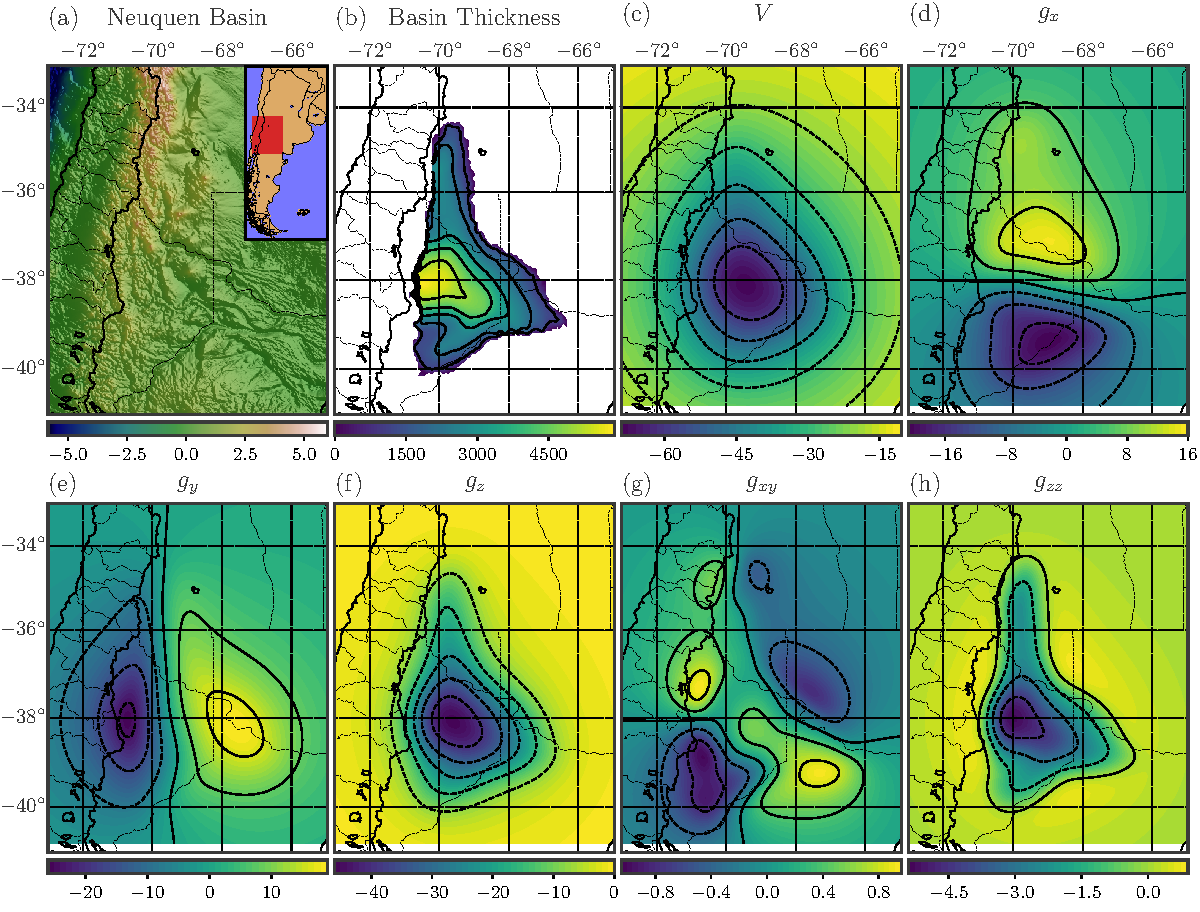
\includegraphics[width=0.975\linewidth]{../manuscript/figures/neuquen-basin.pdf}
\caption{(a) Topography of Neuqu\'en Basin (in km),
         (b) Thickness of the sedimentary basin (in meters),
         (c)-(h) Computed gravity fields: potential $V$ (in J/kg), gradient components $g_x$, $g_y$ and $g_z$ (in mGal) and Marussi tensor components $g_{xy}$ and $g_{zz}$ (in Eötvös), calculated at 50km of height over the ellipsoid.}
\label{fig:neuquen-basin}
\end{figure}

El espesor del paquete sedimentario fue obtenido de \citet{Heine2007}, a partir del cual construimos una grilla regular con una resolución de 0.05$^\circ$ en ambas direcciones latitudinal y longitudinal con un valor de espesor por cada nodo de la grilla (ver Figura \ref{fig:neuquen-basin}b).

Con el objetivo de calcular los campos gravitatorios generados por esta cuenca, hemos creado una malla de tesseroides, cada uno localizado sobre uno de los nodos de la grilla, con dimensiones de 0.05$^\circ$ $\times$ 0.05$^\circ$ y profundidad igual al  espesor de la cuenca en el nodo correspondiente.

Además, tuvimos que definir una función densidad para el modelo completo.
\citet{Sigismondi2012} propuso una densidad mínima y un máxima para la cuenca Nequina de 2755kg/m$^3$ y 412kg/m$^3$, respectivamente.
Para este ejemplo específico hemos escogido una densidad lineal que asume el mínimo en la superficie y el máximo a los 5858m, es decir en la profundidad máxima de la cuenca.

Finalmente hemos realizado el cómputo del potencial gravitatorio, todas las componentes del gradiente ($g_x$, $g_y$, $g_z$) y las componentes $g_{xy}$ y $g_{zz}$ del tensor de Marussi sobre una grilla de cómputo de 159$\times$163 nodos con una separación de 0.05$^\circ$ en ambas direcciones latitudinal y longitudinal, ubicada a 50km de altura sobre el ellipsoide de referencia.
Los campos gravitatorios resultantes pueden observarse en las Figuras \ref{fig:neuquen-basin}c-h.


\bibliographystyle{apalike-es}
\bibliography{../manuscript/bibtex/references}

\end{document}
